
\documentclass{vldb}
\usepackage{graphicx}
\usepackage{balance}
\usepackage[utf8]{inputenc}
\usepackage[spanish]{babel}
% for  \balance command ON LAST PAGE  (only there!)


\begin{document}

% ****************** TITLE ****************************************

\title{LightWeigth Dynamic Memory Managment}

% ****************** AUTHORS **************************************

\numberofauthors{4}

\author{
% 1st. author
\alignauthor
Pablo Rodriguez\\
       \affaddr{Instituto Tecnologico de Costa Rica}\\
       \affaddr{Heredia, Costa Rica}\\
       \email{paroque28@gmail.com}
% 2nd.
\alignauthor
Jiaming Feng\\
       \affaddr{Instituto Tecnologico de Costa Rica}\\
       \affaddr{San Jose, Costa RIca}\\
       \email{alexfengli23@gmail.com}
\and
% 3rd. author
\alignauthor Roberto Bonilla\\
       \affaddr{Instituto Tecnológico de Costa Rica}\\
       \affaddr{Heredia, Costa Rica}\\
       \email{rbj1504@hotmail.com}
}


%%%ABSTRACT


\maketitle

\begin{abstract}
The abstract for your paper for the PVLDB Journal submission.
The template and the example document are based on the ACM SIG Proceedings  templates. This file is part of a package for preparing the submissions for review. These files are in the camera-ready format, but they do not contain the full copyright note.
Note that after the notification of acceptance, there will be an updated style file for the camera-ready submission containing the copyright note.
\end{abstract}


%%%%%%%%%%%%INTRODUCCION

\section{Introduction}
The \textit{proceedings} are the records of a conference.
ACM, as well as PVLDB, seeks to give these conference by-products a uniform,
high-quality appearance.  To do this, ACM / PVLDB has some rigid
requirements for the format of the proceedings documents: there
is a specified format (balanced  double columns), a specified
set of fonts (Arial or Helvetica and Times Roman) in
certain specified sizes (for instance, 9 point for body copy),
a specified live area (18 $\times$ 23.5 cm [7" $\times$ 9.25"]) centered on
the page, specified size of margins (2.54cm [1"] top and
bottom and 1.9cm [.75"] left and right; specified column width
(8.45cm [3.33"]) and gutter size (.083cm [.33"]).

The good news is, with only a handful of manual
settings\footnote{Two of these, the {\texttt{\char'134 numberofauthors}}
and {\texttt{\char'134 alignauthor}} commands, you have
already used; another, {\texttt{\char'134 balancecolumns}}, will
be used in your very last run of \LaTeX\ to ensure
balanced column heights on the last page.}, the \LaTeX\ document
class file handles all of this for you.

The remainder of this document is concerned with showing, in
the context of an ``actual'' document, the \LaTeX\ commands
specifically available for denoting the structure of a
proceedings paper, rather than with giving rigorous descriptions
or explanations of such commands.

%%%%%%%%%%%%%%%%%%%%%%CLASES DISEÑADAS

\section{Clases diseñadas}


%%%%%%%%%%%%%%%%%  vChar
\subsection{class vChar;}


\subsubsection{Ámbito privado}

\subsubsubsection{vRef data;}
referencia en vHeap al dato que contiene la clase


\subsubsection{Ámbito público}

\subsubsubsection{vChar();}
\subsubsubsubsection{Proceso realizado:}
Construye la clase con valor por defecto en 0.

\subsubsubsection{vChar(char);}
\subsubsubsubsection{Parámetros}
char: variable a guardar en vHeap.
\subsubsubsubsection{Proceso realizado:}
Hace un vMalloc para crear la referencia data y un vPlacement para llenarla con el parámetro.

\subsubsubsection{~vChar();}
\subsubsubsubsection{Proceso realizado:}
Destruye la referencia al dato en vHeap.

\subsubsubsection{}
\subsubsubsubsection{}
\subsubsubsubsection{}

\subsubsubsection{}
\subsubsubsubsection{}
\subsubsubsubsection{}

\subsubsubsection{}
\subsubsubsubsection{}
\subsubsubsubsection{}

\subsubsubsection{}
\subsubsubsubsection{}
\subsubsubsubsection{}

\subsubsubsection{}
\subsubsubsubsection{}
\subsubsubsubsection{}

\subsubsubsection{}
\subsubsubsubsection{}
\subsubsubsubsection{}

\subsubsubsection{}
\subsubsubsubsection{}
\subsubsubsubsection{}

\subsubsubsection{}
\subsubsubsubsection{}
\subsubsubsubsection{}

\subsubsubsection{}
\subsubsubsubsection{}
\subsubsubsubsection{}

\subsubsubsection{}
\subsubsubsubsection{}
\subsubsubsubsection{}

\subsubsubsection{}
\subsubsubsubsection{}
\subsubsubsubsection{}

\subsubsubsection{}
\subsubsubsubsection{}
\subsubsubsubsection{}

\subsubsubsection{}

\subsubsubsection{}

\subsubsubsection{}

\subsubsubsection{}

\subsubsubsection{}

\subsubsubsection{}

\subsubsubsection{}


\subsection{class vHeap;}

\subsubsection{Ámbito privado}

\subsubsubsection{friend class Dump;}
Se declara la clase Dump como amiga con el fin eliminar la privacidad entre estas dos clases.
\subsubsubsection{bool* vDebug;}
Puntero a variable booleana que indica si se debe realizar el debug.
\subsubsubsection{int* dumpFrecuency;}
Puntero a variable entera que indica la frecuencia con la que se realizara un dump de memoria.
\subsubsubsection{static vHeap* vHeapSingleton;}
Puntero a vHeap que contiene la única instancia de vHeap.
\subsubsubsection{float* overweight; }
Puntero a variable de punto flotante con valor entre 0 y 1 que corresponde a la sobrecarga de vHeap.
\subsubsubsection{void* mainChunk;}
Abstracción del concepto de heap. Puntero a memoria dinámica que contendrá los datos que el programa requiera almacenar en ejecución.
\subsubsubsection{void* initPos;}
Dirección inicial del mainChunk.
\subsubsubsection{void* finalPos;}
Dirección final del mainChunk.
\subsubsubsection{void* actualPos;}
Dirección actual en el mainChunk, se aumenta cada vez que se reserva memoria con vMalloc y con la desfragmentación y sobrecarga se evita que se salga del mismo.
\subsubsubsection{pthread_mutex_t memoryMutex; }
Mutex de pthread que se utilizará para controlar el acceso a memoria en heap en operaciones delicadas.
\subsubsubsection{vMetaData* metaData;}
Puntero a vMetaData que se utilizará para llevar un control de los datos guardados en el mainChunk.
\subsubsection{Ámbito público}

\subsubsubsection{}

\subsection{}

\subsubsection{Ámbito privado}

\subsubsubsection{}

\subsubsection{Ámbito público}

\subsubsubsection{}


\subsection{Citations}
Citations to articles \cite{bowman:reasoning, clark:pct, braams:babel, herlihy:methodology},
conference
proceedings \cite{clark:pct} or books \cite{salas:calculus, Lamport:LaTeX} listed
in the Bibliography section of your
article will occur throughout the text of your article.
You should use BibTeX to automatically produce this bibliography;
you simply need to insert one of several citation commands with
a key of the item cited in the proper location in
the \texttt{.tex} file \cite{Lamport:LaTeX}.
The key is a short reference you invent to uniquely
identify each work; in this sample document, the key is
the first author's surname and a
word from the title.  This identifying key is included
with each item in the \texttt{.bib} file for your article.

The details of the construction of the \texttt{.bib} file
are beyond the scope of this sample document, but more
information can be found in the \textit{Author's Guide},
and exhaustive details in the \textit{\LaTeX\ User's
Guide}\cite{Lamport:LaTeX}.

This article shows only the plainest form
of the citation command, using \texttt{{\char'134}cite}.
This is what is stipulated in the SIGS style specifications.
No other citation format is endorsed.

\subsection{Tables}
Because tables cannot be split across pages, the best
placement for them is typically the top of the page
nearest their initial cite.  To
ensure this proper ``floating'' placement of tables, use the
environment \textbf{table} to enclose the table's contents and
the table caption.  The contents of the table itself must go
in the \textbf{tabular} environment, to
be aligned properly in rows and columns, with the desired
horizontal and vertical rules.  Again, detailed instructions
on \textbf{tabular} material
is found in the \textit{\LaTeX\ User's Guide}.

Immediately following this sentence is the point at which
Table 1 is included in the input file; compare the
placement of the table here with the table in the printed
dvi output of this document.

\begin{table}
\centering
\caption{Frequency of Special Characters}
\begin{tabular}{|c|c|l|} \hline
Non-English or Math&Frequency&Comments\\ \hline
\O & 1 in 1,000& For Swedish names\\ \hline
$\pi$ & 1 in 5& Common in math\\ \hline
\$ & 4 in 5 & Used in business\\ \hline
$\Psi^2_1$ & 1 in 40,000& Unexplained usage\\
\hline\end{tabular}
\end{table}

To set a wider table, which takes up the whole width of
the page's live area, use the environment
\textbf{table*} to enclose the table's contents and
the table caption.  As with a single-column table, this wide
table will ``float" to a location deemed more desirable.
Immediately following this sentence is the point at which
Table 2 is included in the input file; again, it is
instructive to compare the placement of the
table here with the table in the printed dvi
output of this document.


\begin{table*}
\centering
\caption{Some Typical Commands}
\begin{tabular}{|c|c|l|} \hline
Command&A Number&Comments\\ \hline
\texttt{{\char'134}alignauthor} & 100& Author alignment\\ \hline
\texttt{{\char'134}numberofauthors}& 200& Author enumeration\\ \hline
\texttt{{\char'134}table}& 300 & For tables\\ \hline
\texttt{{\char'134}table*}& 400& For wider tables\\ \hline\end{tabular}
\end{table*}
% end the environment with {table*}, NOTE not {table}!

\subsection{Figures}
Like tables, figures cannot be split across pages; the
best placement for them
is typically the top or the bottom of the page nearest
their initial cite.  To ensure this proper ``floating'' placement
of figures, use the environment
\textbf{figure} to enclose the figure and its caption.

This sample document contains examples of \textbf{.pdf} files to be
displayable with \LaTeX (See Figures \ref{fig:fly} and \ref{fig:bigfly}).  More details on each of these is found in the
\textit{Author's Guide}.

\begin{figure}
\centering

\includegraphics{fly}
\caption{A sample black and white graphic (.pdf format).}
\label{fig:fly}
\end{figure}

\begin{figure}
\centering

\includegraphics[width=1in,height=1in]{fly}
\caption{A sample black and white graphic (.pdf format)
that has been resized with the \texttt{includegraphics} command.}
\label{fig:bigfly}
\end{figure}


As was the case with tables, you may want a figure
that spans two columns.  To do this, and still to
ensure proper ``floating'' placement of tables, use the environment
\textbf{figure*} to enclose the figure and its caption (See Figure~\ref{fig:flies}). And don't forget to end the environment with {figure*}, not {figure}!

\begin{figure*}
\centering
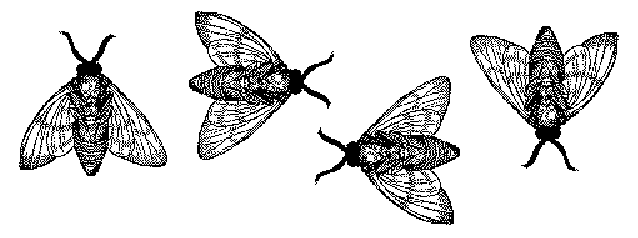
\includegraphics{flies}
\caption{A sample black and white graphic (.pdf format)
that needs to span two columns of text.}
\label{fig:flies}
\end{figure*}


Note that only {\textbf{.pdf}} files were used; if you want to include
{\textbf{.ps}} or {\textbf{.eps}} formats, you can use the
\texttt{{\char'134}epsfig} or \texttt{{\char'134}psfig}
commands as appropriate for the different file types.

\subsection{Theorem-like Constructs}
Other common constructs that may occur in your article are
the forms for logical constructs like theorems, axioms,
corollaries and proofs.  There are
two forms, one produced by the
command \texttt{{\char'134}newtheorem} and the
other by the command \texttt{{\char'134}newdef}; perhaps
the clearest and easiest way to distinguish them is
to compare the two in the output of this sample document:

This uses the \textbf{theorem} environment, created by
the\linebreak\texttt{{\char'134}newtheorem} command:
\newtheorem{theorem}{Theorem}
\begin{theorem}
Let $f$ be continuous on $[a,b]$.  If $G$ is
an antiderivative for $f$ on $[a,b]$, then
\begin{displaymath}\int^b_af(t)dt = G(b) - G(a).\end{displaymath}
\end{theorem}

The other uses the \textbf{definition} environment, created
by the \texttt{{\char'134}newdef} command:
\newdef{definition}{Definition}
\begin{definition}
If $z$ is irrational, then by $e^z$ we mean the
unique number which has
logarithm $z$: \begin{displaymath}{\log e^z = z}\end{displaymath}
\end{definition}

Two lists of constructs that use one of these
forms is given in the
\textit{Author's  Guidelines}.


There is one other similar construct environment, which is
already set up
for you; i.e. you must \textit{not} use
a \texttt{{\char'134}newdef} command to
create it: the \textbf{proof} environment.  Here
is a example of its use:
\begin{proof}
Suppose on the contrary there exists a real number $L$ such that
\begin{displaymath}
\lim_{x\rightarrow\infty} \frac{f(x)}{g(x)} = L.
\end{displaymath}
Then
\begin{align*}
l&=\lim_{x\rightarrow c} f(x)
= \lim_{x\rightarrow c}
\left[ g{x} \cdot \frac{f(x)}{g(x)} \right ] \\
&= \lim_{x\rightarrow c} g(x) \cdot \lim_{x\rightarrow c}
\frac{f(x)}{g(x)} = 0\cdot L = 0,
\end{align*}
which contradicts our assumption that $l\neq 0$.
\end{proof}

Complete rules about using these environments and using the
two different creation commands are in the
\textit{Author's Guide}; please consult it for more
detailed instructions.  If you need to use another construct,
not listed therein, which you want to have the same
formatting as the Theorem
or the Definition\cite{salas:calculus} shown above,
use the \texttt{{\char'134}newtheorem} or the
\texttt{{\char'134}newdef} command,
respectively, to create it.

\subsection*{A {\secit Caveat} for the \TeX\ Expert}
Because you have just been given permission to
use the \texttt{{\char'134}newdef} command to create a
new form, you might think you can
use \TeX's \texttt{{\char'134}def} to create a
new command: \textit{Please refrain from doing this!}
Remember that your \LaTeX\ source code is primarily intended
to create camera-ready copy, but may be converted
to other forms -- e.g. HTML. If you inadvertently omit
some or all of the \texttt{{\char'134}def}s recompilation will
be, to say the least, problematic.

\section{Conclusions}
This paragraph will end the body of this sample document.
Remember that you might still have Acknowledgments or
Appendices; brief samples of these
follow.  There is still the Bibliography to deal with; and
we will make a disclaimer about that here: with the exception
of the reference to the \LaTeX\ book, the citations in
this paper are to articles which have nothing to
do with the present subject and are used as
examples only.
%\end{document}  % This is where a 'short' article might terminate

% ensure same length columns on last page (might need two sub-sequent latex runs)
\balance

%ACKNOWLEDGMENTS are optional
\section{Acknowledgments}
This section is optional; it is a location for you
to acknowledge grants, funding, editing assistance and
what have you.  In the present case, for example, the
authors would like to thank Gerald Murray of ACM for
his help in codifying this \textit{Author's Guide}
and the \textbf{.cls} and \textbf{.tex} files that it describes.


% The following two commands are all you need in the
% initial runs of your .tex file to
% produce the bibliography for the citations in your paper.
\bibliographystyle{abbrv}
\bibliography{vldb_sample}  % vldb_sample.bib is the name of the Bibliography in this case
% You must have a proper ".bib" file
%  and remember to run:
% latex bibtex latex latex
% to resolve all references

\subsection{References}
Generated by bibtex from your ~.bib file.  Run latex,
then bibtex, then latex twice (to resolve references).

%APPENDIX is optional.
% ****************** APPENDIX **************************************
% Example of an appendix; typically would start on a new page
%pagebreak

\begin{appendix}
You can use an appendix for optional proofs or details of your evaluation which are not absolutely necessary to the core understanding of your paper. 

\section{Final Thoughts on Good Layout}
Please use readable font sizes in the figures and graphs. Avoid tempering with the correct border values, and the spacing (and format) of both text and captions of the PVLDB format (e.g. captions are bold).

At the end, please check for an overall pleasant layout, e.g. by ensuring a readable and logical positioning of any floating figures and tables. Please also check for any line overflows, which are only allowed in extraordinary circumstances (such as wide formulas or URLs where a line wrap would be counterintuitive).

Use the \texttt{balance} package together with a \texttt{\char'134 balance} command at the end of your document to ensure that the last page has balanced (i.e. same length) columns.

\end{appendix}



\end{document}
